% Options for packages loaded elsewhere
\PassOptionsToPackage{unicode}{hyperref}
\PassOptionsToPackage{hyphens}{url}
%
\documentclass[
  12pt,
]{article}
\usepackage{lmodern}
\usepackage{setspace}
\usepackage{amssymb,amsmath}
\usepackage{ifxetex,ifluatex}
\ifnum 0\ifxetex 1\fi\ifluatex 1\fi=0 % if pdftex
  \usepackage[T1]{fontenc}
  \usepackage[utf8]{inputenc}
  \usepackage{textcomp} % provide euro and other symbols
\else % if luatex or xetex
  \usepackage{unicode-math}
  \defaultfontfeatures{Scale=MatchLowercase}
  \defaultfontfeatures[\rmfamily]{Ligatures=TeX,Scale=1}
\fi
% Use upquote if available, for straight quotes in verbatim environments
\IfFileExists{upquote.sty}{\usepackage{upquote}}{}
\IfFileExists{microtype.sty}{% use microtype if available
  \usepackage[]{microtype}
  \UseMicrotypeSet[protrusion]{basicmath} % disable protrusion for tt fonts
}{}
\makeatletter
\@ifundefined{KOMAClassName}{% if non-KOMA class
  \IfFileExists{parskip.sty}{%
    \usepackage{parskip}
  }{% else
    \setlength{\parindent}{0pt}
    \setlength{\parskip}{6pt plus 2pt minus 1pt}}
}{% if KOMA class
  \KOMAoptions{parskip=half}}
\makeatother
\usepackage{xcolor}
\IfFileExists{xurl.sty}{\usepackage{xurl}}{} % add URL line breaks if available
\IfFileExists{bookmark.sty}{\usepackage{bookmark}}{\usepackage{hyperref}}
\hypersetup{
  pdftitle={Tidy NEON data for biodiversity research},
  pdfauthor={Daijiang Li1,2†, Sydne Record3†, Eric Sokol4†, Matthew E. Bitters, Melissa Y. Chen, Anny Y. Chung, Matthew Helmus, Ruvi Jaimes, Lara Jansen, Marta A. Jarzyna, Michael G. Just, Jalene M. LaMontagne, Brett Melbourne, Wynne Moss, Kari Norman, Stephanie Parker, Natalie Robinson, Bijan Seyednasrollah, Colin Smith, Sarah Spaulding, Thilina Surasinghe, Sarah Thomsen, Phoebe Zarnetske},
  hidelinks,
  pdfcreator={LaTeX via pandoc}}
\urlstyle{same} % disable monospaced font for URLs
\usepackage[margin=1in]{geometry}
\usepackage{longtable,booktabs}
% Correct order of tables after \paragraph or \subparagraph
\usepackage{etoolbox}
\makeatletter
\patchcmd\longtable{\par}{\if@noskipsec\mbox{}\fi\par}{}{}
\makeatother
% Allow footnotes in longtable head/foot
\IfFileExists{footnotehyper.sty}{\usepackage{footnotehyper}}{\usepackage{footnote}}
\makesavenoteenv{longtable}
\usepackage{graphicx}
\makeatletter
\def\maxwidth{\ifdim\Gin@nat@width>\linewidth\linewidth\else\Gin@nat@width\fi}
\def\maxheight{\ifdim\Gin@nat@height>\textheight\textheight\else\Gin@nat@height\fi}
\makeatother
% Scale images if necessary, so that they will not overflow the page
% margins by default, and it is still possible to overwrite the defaults
% using explicit options in \includegraphics[width, height, ...]{}
\setkeys{Gin}{width=\maxwidth,height=\maxheight,keepaspectratio}
% Set default figure placement to htbp
\makeatletter
\def\fps@figure{htbp}
\makeatother
\setlength{\emergencystretch}{3em} % prevent overfull lines
\providecommand{\tightlist}{%
  \setlength{\itemsep}{0pt}\setlength{\parskip}{0pt}}
\setcounter{secnumdepth}{-\maxdimen} % remove section numbering
\usepackage{geometry}
\geometry{verbose,letterpaper,margin=2.45cm}

% \usepackage[breaklinks=true,pdfstartview=FitH,citecolor=blue]{hyperref}
\hypersetup{colorlinks,%
	citecolor=blue,%
	filecolor=red,%
	linkcolor=blue,%
	urlcolor=red,%
	pdfstartview=FitH}

% \usepackage[T1]{fontenc}
% \usepackage[utf8]{inputenc}
% \usepackage{textgreek}
% \usepackage{babel}
\usepackage{microtype}
\usepackage{amsmath}
\usepackage[osf]{libertine}
\usepackage{libertinust1math}
\usepackage{inconsolata}

\usepackage{booktabs}

% \usepackage{setspace}
% \doublespacing

% \setstretch{1.8999999999999999}

\usepackage{lineno}
\linenumbers

\usepackage{authblk}
\renewcommand\Authfont{\fontsize{10.5}{11}\selectfont}

\usepackage{caption}
% \DeclareCaptionLabelSeparator{bar}{\textbf{ | }}
% \captionsetup{
%    labelsep=bar
% }

% \renewcommand{\rmdefault}{cmr}


% flush left while keep identation
\makeatletter
\newcommand\iraggedright{%
  \let\\\@centercr\@rightskip\@flushglue \rightskip\@rightskip
  \leftskip\z@skip}
\makeatother
\raggedright

% make pdf as default figure format
\DeclareGraphicsExtensions{.pdf,.png, %
    .jpg,.mps,.jpeg,.jbig2,.jb2,.JPG,.JPEG,.JBIG2,.JB2}
\usepackage{booktabs}
\usepackage{longtable}
\usepackage{array}
\usepackage{multirow}
\usepackage{wrapfig}
\usepackage{float}
\usepackage{colortbl}
\usepackage{pdflscape}
\usepackage{tabu}
\usepackage{threeparttable}
\usepackage{threeparttablex}
\usepackage[normalem]{ulem}
\usepackage{makecell}
\newlength{\cslhangindent}
\setlength{\cslhangindent}{1.5em}
\newenvironment{cslreferences}%
  {\setlength{\parindent}{0pt}%
  \everypar{\setlength{\hangindent}{\cslhangindent}}\ignorespaces}%
  {\par}

\title{Tidy NEON data for biodiversity research}
\author{Daijiang Li\textsuperscript{1,2†}, Sydne Record\textsuperscript{3†}, Eric Sokol\textsuperscript{4†}, Matthew E. Bitters, Melissa Y. Chen, Anny Y. Chung, Matthew Helmus, Ruvi Jaimes, Lara Jansen, Marta A. Jarzyna, Michael G. Just, Jalene M. LaMontagne, Brett Melbourne, Wynne Moss, Kari Norman, Stephanie Parker, Natalie Robinson, Bijan Seyednasrollah, Colin Smith, Sarah Spaulding, Thilina Surasinghe, Sarah Thomsen, Phoebe Zarnetske}
\date{09 December, 2020}

\begin{document}
\maketitle

% align only at left, not at right.
\iraggedright

\setstretch{1.5}
\textbf{Abstract}: Authors of this paper are all interested in using NEON data for biodiversity research. We have spent lots of time reading the documentations and cleaning up the data for our own studies. We believe that we can document our data cleaning process and provide the tidy NEON data for the community so that others can use the data readily for biodiversity research.

\textbf{Key words}: NEON, Biodiversity, Data

\hypertarget{introduction-or-why-tidy-neon-data}{%
\section{Introduction (or why tidy NEON data)}\label{introduction-or-why-tidy-neon-data}}

A central goal of ecology is to understand the patterns and processes of biodiversity, which is particularly important in an era of rapid global environmental change (Midgley and Thuiller \protect\hyperlink{ref-midgley2005global}{2005}, Blowes et al. \protect\hyperlink{ref-blowes2019geography}{2019}). Such understanding comes from addressing questions like: How is biodiversity distributed across large spatial scales, ranging from ecoregions to continents? What mechanisms drive spatial patterns of biodiversity? Are spatial patterns of biodiversity similar among different taxonomic groups, and if not, why do we see variation? How does community composition vary across geographies? What are the local and landscape scale drivers of community structure? How and why do biodiversity patterns change over time? Answers to such questions are essential to understanding, managing, and conserving biodiversity and the ecosystem services it influences.

Biodiversity research has a long history (Worm and Tittensor \protect\hyperlink{ref-worm2018theory}{2018}), beginning with major scientific expeditions (e.g., Alexander von Humboldt, Charles Darwin) that were undertaken to explore global biodiversity after the establishment of Linnaeus's Systema Naturae (Linnaeus \protect\hyperlink{ref-linnaeus1758systema}{1758}). Modern biodiversity research dates back to the 1950s (Curtis \protect\hyperlink{ref-curtis1959vegetation}{1959}, Hutchinson \protect\hyperlink{ref-hutchinson1959homage}{1959}) and aims to quantify patterns of species diversity and describe mechanisms underlying its heterogeneity. Since the beginning of this line of research, major theoretical breakthroughs (MacArthur and Wilson \protect\hyperlink{ref-macarthur1967theory}{1967}, Hubbell \protect\hyperlink{ref-hubbell2001unified}{2001}, Brown et al. \protect\hyperlink{ref-brown2004toward}{2004}) have advanced our understanding of potential mechanisms causing and maintaining biodiversity. Modern empirical studies, however, have been largely constrained to local or regional scales, and focused on one or a few specific taxonomic groups. Despite such constraints, field ecologists have compiled unprecedented numbers of observations, which support research into generalities through syntheses and meta-analyses (Vellend et al. \protect\hyperlink{ref-vellend2013global}{2013}, Blowes et al. \protect\hyperlink{ref-blowes2019geography}{2019}, Li et al. \protect\hyperlink{ref-li2020changes}{2020}). Such work is challenged, however, by the difficulty of bringing together data from different studies and with varying limitations, including: differing collection methods (methodological uncertainties); varying levels of statistical robustness; inconsistent handling of missing data; spatial bias; publication bias; and design flaws (Martin et al. \protect\hyperlink{ref-martin2012mapping}{2012}, Nakagawa and Santos \protect\hyperlink{ref-nakagawa2012methodological}{2012}, Koricheva and Gurevitch \protect\hyperlink{ref-koricheva2014uses}{2014}). Additionally, it has historically been challenging for researchers to obtain and collate data from a diversity of sources, for use in syntheses and/or meta-analyses (Gurevitch and Hedges \protect\hyperlink{ref-gurevitch1999statistical}{1999}). This has been remedied in recent years by large efforts to digitize museum and herbarium specimens (e.g., iDigBio), successful community science programs (e.g., iNaturalist, eBird), and advances in technology (e.g., remote sensing, automated acoustic recorders) that together bring biodiversity research into the big data era (Hampton et al. \protect\hyperlink{ref-hampton2013big}{2013}, Farley et al. \protect\hyperlink{ref-farley2018situating}{2018}). Yet, each of these comes with its own limitations. For example, museum/herbarium specimens and community science records are incidental (thus, unstructured in terms of the sampling design) and show obvious geographic and taxonomic biases (Martin et al. \protect\hyperlink{ref-martin2012mapping}{2012}, Beck et al. \protect\hyperlink{ref-beck2014spatial}{2014}, Geldmann et al. \protect\hyperlink{ref-geldmann2016determines}{2016}); remote sensing approaches can cover large spatial scales, but may be of low spatial resolution and unable to reliably penetrate vegetation canopy (Palumbo et al. \protect\hyperlink{ref-palumbo2017building}{2017}, G Pricope et al. \protect\hyperlink{ref-g2019remote}{2019}). Overall, our understanding of biodiversity is currently limited by the lack of standardized high quality and open-access data across large spatial scales and long time periods.

There is currently a major effort underway to overcome the issues above. For example, the Long Term Ecological Research Network (LTER) consists of 28 sites that provide long term datasets for a diverse set of ecosystems. However, there is no standardization in the design and data collections across LTER sites. The National Ecological Observatory Network (NEON) is a continental-scale observatory network that collects long-term, standardized, and open access datasets broadly aimed at enabling better understanding of how U.S. ecosystems change through time (Keller et al. \protect\hyperlink{ref-keller2008continental}{2008}). Data collected include observations and field surveys, automated instrument measurements, airborne remote sensing surveys, and archival samples that characterize plants, animals, soils, nutrients, freshwater and atmospheric conditions. Data are collected at 81 field sites across both terrestrial and freshwater ecosystems across the United States and will continue for 30 years. These data provide a unique opportunity for advancing biodiversity research because consistent data collection protocols and the long-term nature of the observatory ensure sustained data availability and directly comparable measurements across locations. Spatio-temporal patterns in biodiversity, and the causes of changes to these patterns, can thus be confidently assessed and analyzed using NEON data.

NEON data are designed to be maximally useful to ecologists by aligning with FAIR principles (findable, accessible, interoperable, and reusable Wilkinson et al. \protect\hyperlink{ref-wilkinson2016fair}{2016}), but there are still hurdles to overcome in the use of their organismal data for biodiversity research. For example, different NEON data products use different field names for similar measurements, some include sampling unit information while this must be calculated for others, etc. Furthermore, NEON organismal data products provide lots of raw data, most of them may not be needed to calculate biodiversity measurements. Therefore, users need to dive into the comprehensive documentation to better understand the organismal datasets, to extract the relevant essential variables, and to take additional steps to quantify biodiversity (e.g., clean datasets, change the data formats to feed the data to statistical programs, etc.). Such processes can be very time consuming and the path to get to that standard data format is different and not always obvious for each NEON organismal data product. A data product that simplifies and standardizes various NEON organismal datasets can remove such hurdles, enhance the interoperability and reusability, and facilitate wider usage of NEON organismal datasets for biodiversity research.

Here, our goal is to provide a standardized ``tidy version'' of NEON organismal datasets for Biodiversity research. Users can download the tidy data from the R package ecocomDP (CITATION), which will be maintained and updated when new data is available from the NEON portal. Our hope is to standardize formats across NEON data products and substantially reduce data cleaning times for the large ecology community, and to facilitate the use of NEON data to advance biodiversity research.

\hypertarget{materials-and-methods-or-how-to-tidy-neon-organismal-data}{%
\section{Materials and Methods (or how to tidy NEON organismal data)}\label{materials-and-methods-or-how-to-tidy-neon-organismal-data}}

General points we could go over that apply to all data sets before going into details:

\hypertarget{terrestrial-organisms}{%
\subsection{Terrestrial Organisms}\label{terrestrial-organisms}}

\hypertarget{breeding-land-birds}{%
\subsubsection{Breeding Land Birds}\label{breeding-land-birds}}

\textbf{NEON Sampling Design} Landbirds are surveyed with point counts during the breeding season in each of the 47 terrestrial sites, co-located with distributed plots whenever possible (Fig. 1). Breeding landbirds are ``smaller birds (usually exclusive of raptors and upland game birds) not usually associated with aquatic habitats'' (Ralph et al.~1993). At NEON sites, one sampling bout occurs per breeding season at large sites, and two sampling bouts occur at smaller sites. Point counts occur either within randomly distributed individual points or within bird grids at each site in representative (dominant) vegetation. At large NEON sites, 5-15 grids are sampled with nine point count locations each, where grid centers are co-located with distributed base plot centers, if possible. If small sites only allow five grids, a stratified random sample maintains 250 m minimum separation between point count locations and point counts occur at the southwest corner of the 5-25 distributed base plots.

The breeding season month, which defines the timing of sampling, varies somewhat by site but always occurs in the spring. Most species observed are diurnal and include both resident and migrant species. Early in the morning observers conduct point counts wherein the observer tracks each minute. Each point count contains species, sex, and distance to each bird (measured with a laser rangefinder except in the case of flyovers) seen or heard during a 6-minute period after a 2-minute acclimation period. To enable subsequent modeling of detectability, additional data collected during the point counts include: weather, distances from observers to birds, and the detection methods. The point count surveys for NEON were modified from the Integrated Monitoring in Bird Conservation Regions (IMBCR): Field protocol for spatially-balanced sampling of landbird populations (Pavlacky Jr et al. \protect\hyperlink{ref-pavlacky2017statistically}{2017}).

To protect species of concern, their taxonomic IDs are `fuzzed.' This means the data are provided with a taxonomic identification at one higher taxonomic level than where the protection occurs. For example, if a threatened Black-capped vireo (Vireo atricapilla) is recorded by a NEON technician, the taxonomic identification is fuzzed to Vireo in the data. Rare, threatened and endangered species are those listed as such by federal and/or state agencies.

\textbf{Data Wrangling Decisions} Bird point count data (`DP1.10003.001'), consist of a list of two associated data frames: \texttt{brd\_countdata} and \texttt{brd\_perpoint}). The former data frame contains information such as locations, species identities, and their counts. The second data frame contains additional location information such as latitude longitude coordinates and environmental conditions during the time of the observations. It is relatively straightforward to prepare the bird point count data for biodiversity research. We first combined both data frames into one and then removed columns that are likely not needed (e.g., laboratory names, publication dates, etc.).

\hypertarget{ground-beetles}{%
\subsubsection{Ground Beetles}\label{ground-beetles}}

\textbf{NEON Sampling Design} Each site is sampled via pitfall trap, with 10 separate distributed plots at each site and four pitfall traps at each plot initially - placed in the ground at the cardinal direction points of the distributed plot boundary. This equates to a total of 40 pitfall traps per site. In 2018, sampling was reduced via the elimination of the North pitfall trap in each plot, resulting in 30 traps per site. Sampling begins when the temperature has been \textgreater4°C for 10 days in the spring and ends when temperatures dip below this threshold in the fall. Sampling occurs biweekly throughout the sampling season with no single trap being sampled more frequently than every 12 days. After collection, the samples are separated into carabid species and bycatch, with bycatch archived at either the trap (vertebrate) or plot (invertebrate) level. Carabid samples are sorted and identified by NEON technicians, after which a subset of individuals are sent to be pinned and re-identified by an expert taxonomist.

\textbf{Data Wrangling Decisions} Beetle samples are identified at multiple levels of expertise. Beetles are first identified by the sorting technician and then the pinning technician. Identifications of more difficult specimens are additionally verified by an expert taxonomist. Whenever available, expert identification was used for a sample. For example, if taxonomic delineation between NEON staff and multiple expert taxonomist identifications do not agree, then the consensus expert taxonomist delineation is recorded in the data portal.

Beetle abundances are recorded on the sorted sample, by NEON technicians, and are not preserved across the different levels of identification. For example, a sample of 15 individuals identified during the sorting phase may be passed to a pinning technician, who then identifies five different species within that sample. The pinning technician does not back annotate the sorted sample to identify which individuals are which species, or go through and re-identify the rest of the individuals in the sample. Without this, we have assumed that all individuals in the sorted sample that were not positively identified by an expert were correctly identified in the original sample by NEON technicians. Hence, the abundance for a newly identified species is one, and the abundance for the originally identified species for the sample is the original abundance minus the individuals expertly identified as a different species.

Sometimes there are more individuals identified by pinning technicians or experts than were counted in the original sorted sample, so the count has been updated in the dataset. There are also a few cases where an especially difficult identification was sent to multiple expert taxonomists and they did not agree on a final taxon, these individuals were excluded from the data set at the recommendation of NEON staff.

Prior to 2018, \texttt{trappingDays} values were not included for many sites. Missing entries were calculated as the range from \texttt{setDate} through \texttt{collectDate} for each trap. We also account for a few plots for which \texttt{setDate} was not updated based on a previous collection event in the \texttt{trappingDays} calculations. To facilitate easy manipulation of data within and across bouts a new \texttt{boutID} field was created to identify all trap collection events at a site in a bout. The original \texttt{EventID} field is intended to identify a bout, but has a number of issues that necessitates creation of a new ID. First, \texttt{EventID} does not correspond to a single collection date but rather all collections in a week. This is appropriate for the small number of instances when collections for a bout happen over multiple consecutive days (\textasciitilde5\% of bouts), but prevents analysis of bout patterns at the temporal scale of a weekday. The data here were updated so all entries for a bout correspond to the date (i.e., \texttt{collectDate}) on which the majority of traps are collected in order to maintain the weekday-level resolution with as high of fidelity as possible, while allowing for easy aggregation within bouts and \texttt{collectDate}'s. Second, there were a few instances in which plots within a site were set and collected on the same day, but have different \texttt{EventID}'s. These instances were all considered a single bout by our new \texttt{boutID}, which is a unique combination of \texttt{setDate}, \texttt{collectDate}, and \texttt{siteID}.

\hypertarget{mosquitos}{%
\subsubsection{Mosquitos}\label{mosquitos}}

\textbf{NEON Sampling Design} Mosquito specimens are collected at 47 terrestrial sites across all NEON domains. Traps are distributed throughout the site according to a stratified-random spatial design used for all Terrestrial Observation System sampling, and are typically located within 30m of a road to facilitate expedient sampling. NEON collects mosquito specimens using the Center for Disease Control (CDC) CO\textsubscript{2} light traps. These traps have been used by other public health and mosquito-control agencies for a half-century, which allows NEON mosquito data to be used across field sites and in combination with existing long-term data sets. A CDC CO\textsubscript{2} light trap consists of a cylindrical insulated cooler that contains dry ice, a plastic rain cover attached to a light/fan assembly (battery powered), and a mesh collection cup. During deployment, the dry ice sublimates and releases CO\textsubscript{2}. Mosquitoes attracted to the CO\textsubscript{2} bait are sucked into the mesh collection cup by the battery-powered fan, where they remain alive until the trap is collected.

Mosquito monitoring is divided into field season and off-season sampling. Off-season sampling takes place weekly at core sites, and begins after three consecutive zero-catch field sampling bouts at a core site. The goal of off-season sampling is to rapidly determine when the next field season should begin and to provide mosquito phenology data throughout the lifetime of the observatory. During the off season, overnight sampling occurs weekly at three dedicated mosquito plots spread throughout the terrestrial core sites for each domain, only if temperatures are above 10 °C. Traps are deployed at dusk and checked the following dawn. Field season sampling begins when the first mosquito is detected during off season sampling. Technicians collect samples every two weeks at core terrestrial sites and every four weeks at relocatable terrestrial sites. Sampling occurs at 10 dedicated mosquito plots at each site over a 24-hour period, or one sampling bout. During the sampling bout, traps are serviced twice and yield one night-active sample, taken at dawn or about 8 hours after trap is set, and one day-active sample, taken at dusk or about 16 hours after the trap is set. Thus, a 24-hour sampling bout yields 20 ``samples'' from ten traps.

Following field collection, NEON's field ecologists process, pack up and ship the samples to an external lab where mosquitoes are identified to species and sex (when possible). A subset of identified mosquitoes are tested for infection by pathogens to quantify the presence/absence and prevalence of various arboviruses. Some mosquitoes are set aside for DNA barcode analysis as well as long-term archiving. Particularly rare or difficult to identify mosquito specimens are prioritized for DNA barcoding.

\textbf{Data Wrangling Decisions} Mosquito data are mainly stored in four data frames: trapping data (\texttt{mos\_trapping}), sorting data (\texttt{mos\_sorting}), archiving data (\texttt{mos\_archivepooling}), and expert taxonomist processed data (\texttt{mos\_expertTaxonomistIDProcessed}). We first removed rows (records) with missing important information about location, collect date, and sample or subsample ID for all data frames. We then merged all four data frames into one while checked carefully during the process. In the merged data frame, we only kept records that have target taxa (i.e., \texttt{targetTaxaPresent\ ==\ "Y"}) or have no known compromised sampling condition (i.e., \texttt{sampleCondition\ ==\ "No\ known\ compromise"}). We further removed a small number of records with species identified at family level; all remaining records were identified at least at the genus level. We estimated the total individual count for each species within a trap as \texttt{individualCount\ *\ (totalWeight\ /\ subsampleWeight)}. We then removed columns that likely will not be used for calculating biodiversity values.

\hypertarget{small-mammals}{%
\subsubsection{Small Mammals}\label{small-mammals}}

\textbf{NEON Sampling Design} NEON defines small mammals based on taxonomic, behavioral, dietary, and size constraints, and includes any rodent that is (1) nonvolant; (2) nocturnally active; (3) forages predominantly aboveground; and (4) has a mass \textgreater5 grams, but \textless{} about 500-600 g (Thibault et al.~2019). In North America, this includes cricetids, heteromyids, small sciurids, and introduced murids, but excludes shrews, large squirrels, rabbits, or weasels, despite the fact that individuals of these species may be incidentally captured. A total of 65 species across the US meet these criteria and are designated as ``target species'\,'. Small mammals are collected at NEON sites using Sherman traps, identified to species in the field, marked with a unique tag, and released. Multiple 90 m x 90 m trapping grids are set up in each terrestrial field site within the dominant vegetation type. Each 90 m x 90 m trapping grid contains 100 traps placed in a pattern with ten rows and ten columns set 10 m apart. Three 90 m x 90 m grids per site are designated pathogen grids and the remainder are designated diversity grids. Small mammal sampling occurs in bouts, with a bout comprised of three consecutive (or nearly consecutive) nights of trapping, and is based on the lunar calendar, with timing of sampling constrained to occur within 10 days before or after the new moon. The number of bouts per year is determined by site type, and most sites contain six bouts per year.

\textbf{Data Wrangling Decisions} In the data presented, records are stratified by NEON site, year, month, and day. Capture records were removed if they were not identified to genus or species (e.g., if the species name was denoted as `either/or' or as family name). Records were also removed if they represented dead animals (fate=`dead') or, escaped animals (fate=`escaped'), or bycatch (fate=`nontarget', i.e., non-target species). Records for recaptured individuals were also removed. However, we kept empty traps as they contain information about sampling efforts, which can be useful for some studies.

\hypertarget{soil-microbes}{%
\subsubsection{Soil Microbes}\label{soil-microbes}}

\textbf{NEON Sampling Design} Soil samples are collected at ten 40 x 40 m\textsuperscript{2} NEON plots per site. Four plots are within the tower airshed (tower plots), and six plots are distributed across the landscape (gradient plots). At each sampling time point, soils are sampled from three of the four subplots, and one total sample collected from a randomly-generated XY coordinate location within each subplot. At each sampling location, soils are taken at the surface horizon most years, but from both organic and mineral horizons every five years during coordinated microbe/biogeochemistry bouts. Most sites, except for the boreal/arctic sites, are sampled three times a year, once at peak vegetation greenness and two other times bracketing that period. This results in \textasciitilde10 plots * 3 locations * 1 or 2 horizons * 3 periods = 90 - 180 soil samples per site per year for most sites. Samples for microbial biomass, composition, and metagenomics are stored on dry ice and shipped to an external lab (variable depending on year) for downstream processing.

\textbf{Data Wrangling Decisions} Unlike other NEON biodiversity data, the soil microbial datasets require significant pre-processing to go from raw sequence data to a community matrix, and the exact bioinformatics methods will vary depending on use case. Briefly, major decisions during this process will depend on whether users are working with fungal (ITS) or bacterial (16S) data, if the goal is to maximize read quality and taxonomic resolution vs.~number of reads retained through the quality filter process, and whether to remove or retain reverse complement reads for a merged sequence. The full description of a suggested bioinformatics pipeline, how to run sensitivity analyses on user-defined parameters, accompanying code, and vignettes are described in Qin et al in this issue. At the end of the suggested bioinformatics pipeline, users will have a phyloseq object, which is a commonly-used format for sequence-based analysis software. The phyloseq object will contain a table of ASV (amplicon sequence variant) sequences, a table of taxonomic assignments, and soil chemical and physical data associated with the same sample locations and sampling bouts.

\hypertarget{terrestrial-plants}{%
\subsubsection{Terrestrial Plants}\label{terrestrial-plants}}

\textbf{NEON Sampling Design} NEON plant diversity plots sampled during one or two bouts per year, and are a total of 400 m x 400 m. Sampling is done using a nested design, where the entire plot is first subdivided into 4 100 m x 100 m subplots. For each of these, one or more 1 m x 1 m nested subplots are then sampled; species coverages within the 1 m\textsuperscript{2} area were estimated visually. Next, one or more 10 m x 10 m subplots, inside of which the finer resolution subplots are located, are sampled. Finally, the 100 m x 100 m subplot is sampled. At 10 m by 10 m and 100 m by 100 m scales, only presence and absence of plants were recorded. Each species is recorded only once during sampling, such that an observation of a species at a fine-resolution subplot prevents it from being recorded again if it is encountered in a coarser scale subplot. A full dataset for each NEON plant diversity plot was generated by combining all data from all subplots within the 400 m x 400 m boundary, and removing duplicates (which may occur across the 100 m x 100 m subdivisions). More details about the sampling design can be found in Barnett et al. (\protect\hyperlink{ref-barnett2019plant}{2019}).

NEON manages plant taxonomic entries with a master taxonomy list that is based on the community standard, where possible. Using this list, synonyms for a given species are converted to the currently used name. The master taxonomy for plants is the USDA PLANTS Database (USDA, NRCS. 2014. \url{https://plants.usda.gov}), and the portions of this database included in the NEON plant master taxonomy list are those pertaining to native and naturalized plants present in NEON sampling area. A sublist for each NEON domain includes those species with ranges that overlap the domain as well as nativity designations - introduced or native - in that part of the range. If a species is reported at a location outside of its known range, and the record proves reliable, the master taxonomy list is updated to reflect the distribution change. For more on the NEON plant master taxonomy list see \href{https://data.neonscience.org/api/v0/documents/NEON.DOC.014042vK}{NEON.DOC.014042}.

\textbf{Data Wrangling Decisions} Because sampling at the 1 m x 1 m scale also includes observations of abiotic and non-target species ground cover (i.e., soil, water, downed wood, etc), we removed records with \texttt{divDataType} as ``otherVariables''. We also removed records whose \texttt{targetTaxaPresent} is \texttt{N} (i.e., non a target species). Additionally, for all spatial resolution with observatory data (i.e., 1 m x 1 m, 10 m x 10 m, and 100 m x 100 m data), any record lacking information critical to combining data within a plot and for a given sampling bout (i.e., \texttt{plotID}, \texttt{subplotID}, \texttt{boutNumber}, \texttt{endDate}, or \texttt{taxonID}) was dropped from the dataset. Furthermore, records without a definitive genus or species level \texttt{taxonID} (i.e., those representing unidentified morphspecies) were not considered. To stack data from different spatial resolution into one data frame, we created a pivot column named as \texttt{sample\_area\_m2} (possible values are 1, 100, and 10000). Because of the nested design of plant data, to get all records within a subplot at 10 m by 10 m scale, we need to use all data from both 1 m by 1 m and 10 m by 10 m scales for that subplot; similarly, to get all records within a subplot at 100 m by 100 m scale, we need to include all data from that subplot. Species abundance information was only recorded as area coverage within 1 m by 1 m subplots; however, users may use the frequency of a species across subplots within a plot or plots within a site as a proxy of its abundance if needed.

\hypertarget{ticks}{%
\subsubsection{Ticks}\label{ticks}}

\textbf{NEON Sampling Design}

\textbf{Data Wrangling Decisions}

\hypertarget{tick-pathogens}{%
\subsubsection{Tick pathogens}\label{tick-pathogens}}

\textbf{NEON Sampling Design}

\textbf{Data Wrangling Decisions}

\hypertarget{aquatic-organisms}{%
\subsection{Aquatic Organisms}\label{aquatic-organisms}}

\hypertarget{microalgae-periphyton-and-phytoplankton}{%
\subsubsection{MicroAlgae (Periphyton and Phytoplankton)}\label{microalgae-periphyton-and-phytoplankton}}

\textbf{NEON Sampling Design}

\textbf{Data Wrangling Decisions}

\hypertarget{fish}{%
\subsubsection{Fish}\label{fish}}

\textbf{NEON Sampling Design}

\textbf{Data Wrangling Decisions}

\hypertarget{aquatic-macroinvertebrates}{%
\subsubsection{Aquatic macroinvertebrates}\label{aquatic-macroinvertebrates}}

\textbf{NEON Sampling Design}

\textbf{Data Wrangling Decisions}

\hypertarget{results-or-how-to-get-and-use-tidy-neon-organismal-data}{%
\section{Results (or how to get and use tidy NEON organismal data)}\label{results-or-how-to-get-and-use-tidy-neon-organismal-data}}

All cleaned data products can be obtained from the R package \texttt{neonDivData}, which can be installed from Github. Installation instructions can be found on the Github webpage (\url{https://github.com/daijiang/neonDivData}). Table \ref{tab:dataSummary} shows the brief summary of all data products. To get a specific data product, we can just call the objects in the \texttt{data\_product} column in Table x. Such data products include cleaned (and standardized if needed) occurrence data for the taxonomic groups covered. If environmental information and species measurements were provided by NEON for some taxonomic groups, they are also included in these data products. Information such as latitude, longitude, and elevation for all taxonomic groups were saved in the \texttt{neon\_locations} object of the R package. Information about species scientific names and identification references of all taxonomic groups were saved in the \texttt{neon\_taxa} object.



\begin{table}

\caption{\label{tab:dataSummary}\textbf{Summary of data products included in this study.}}
\centering
\resizebox{\linewidth}{!}{
\begin{tabular}[t]{lllrrrrl}
\toprule
taxa & neon\_DPI & data\_product & n\_site & n\_species & start\_year & end\_year & modify\_time\\
\midrule
\cellcolor{gray!6}{algae} & \cellcolor{gray!6}{DP1.20166.001} & \cellcolor{gray!6}{data\_algae} & \cellcolor{gray!6}{33} & \cellcolor{gray!6}{1824} & \cellcolor{gray!6}{2014} & \cellcolor{gray!6}{2019} & \cellcolor{gray!6}{2020-10-30}\\
beetle & DP1.10022.001 & data\_beetle & 47 & 756 & 2013 & 2020 & 2020-11-10\\
\cellcolor{gray!6}{bird} & \cellcolor{gray!6}{DP1.10003.001} & \cellcolor{gray!6}{data\_bird} & \cellcolor{gray!6}{47} & \cellcolor{gray!6}{535} & \cellcolor{gray!6}{2013} & \cellcolor{gray!6}{2019} & \cellcolor{gray!6}{2020-11-23}\\
fish & DP1.20107.001 & data\_fish & 27 & 125 & 2016 & 2020 & 2020-11-11\\
\cellcolor{gray!6}{macroinvertebrate} & \cellcolor{gray!6}{DP1.20120.001} & \cellcolor{gray!6}{data\_macroinvertebrate} & \cellcolor{gray!6}{34} & \cellcolor{gray!6}{1276} & \cellcolor{gray!6}{2014} & \cellcolor{gray!6}{2020} & \cellcolor{gray!6}{2020-10-30}\\
mosquito & DP1.10043.001 & data\_mosquito & 47 & 126 & 2015 & 2020 & 2020-10-30\\
\cellcolor{gray!6}{plant} & \cellcolor{gray!6}{DP1.10058.001} & \cellcolor{gray!6}{data\_plant} & \cellcolor{gray!6}{47} & \cellcolor{gray!6}{6075} & \cellcolor{gray!6}{2013} & \cellcolor{gray!6}{2020} & \cellcolor{gray!6}{2020-10-30}\\
small\_mammal & DP1.10072.001 & data\_small\_mammal & 46 & 145 & 2014 & 2019 & 2020-10-30\\
\cellcolor{gray!6}{tick} & \cellcolor{gray!6}{DP1.10093.001} & \cellcolor{gray!6}{data\_tick} & \cellcolor{gray!6}{41} & \cellcolor{gray!6}{19} & \cellcolor{gray!6}{2014} & \cellcolor{gray!6}{2018} & \cellcolor{gray!6}{2020-10-30}\\
tick\_pathogen & DP1.10092.001 & data\_tick\_pathogen & 14 & 12 & 2013 & 2020 & 2020-10-30\\
\bottomrule
\end{tabular}}
\end{table}

To demonstrate the use of data products, we used \texttt{data\_plant} to quickly visualize the distribution of species richness of plants across all NEON sites (Fig. \ref{fig:Fig2Map}). To show how easy it is to get site level species richness, we presented the code used to generate the data for Fig. \ref{fig:Fig2Map} below.



\begin{figure}

{\centering 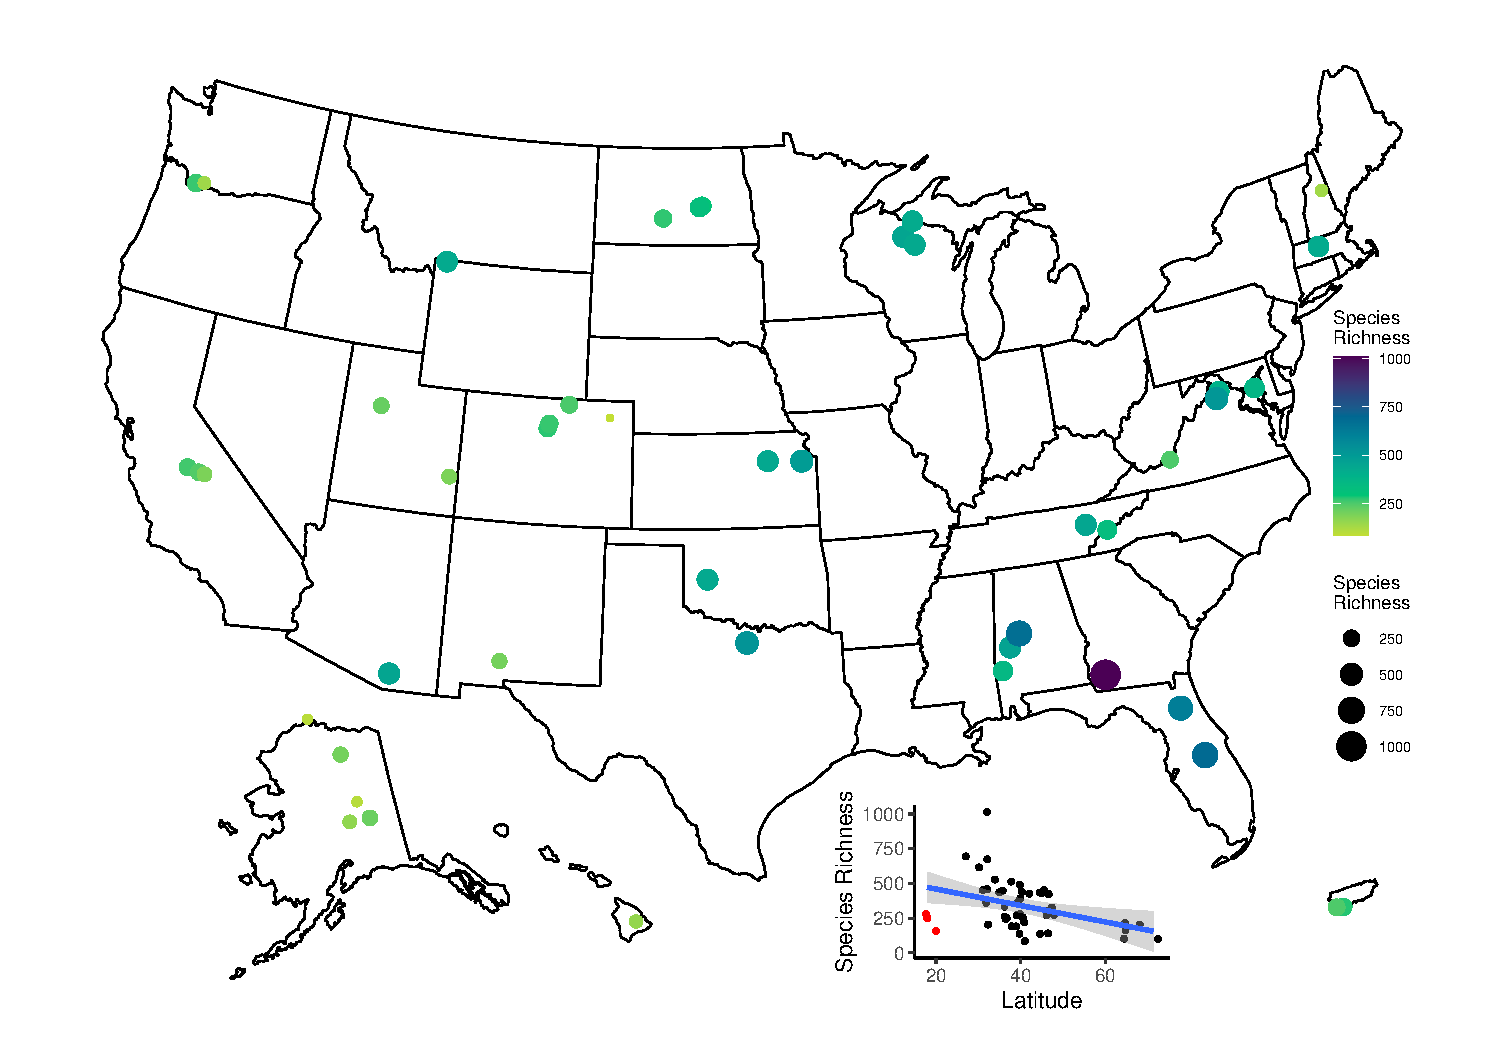
\includegraphics[width=0.95\linewidth]{/Users/dli/Github/neonDivData/manuscript/figures/p_plant} 

}

\caption{Distribution of plant species richness across all NEON terrestrial sites. Alaska, Hawaii, and Puerto Rico were rearranged to save space.}\label{fig:Fig2Map}
\end{figure}

\hypertarget{reference}{%
\section*{Reference}\label{reference}}
\addcontentsline{toc}{section}{Reference}

\hypertarget{refs}{}
\begin{cslreferences}
\leavevmode\hypertarget{ref-barnett2019plant}{}%
Barnett, D. T., P. B. Adler, B. R. Chemel, P. A. Duffy, B. J. Enquist, J. B. Grace, S. Harrison, R. K. Peet, D. S. Schimel, T. J. Stohlgren, and others. 2019. The plant diversity sampling design for the national ecological observatory network. Ecosphere 10:e02603.

\leavevmode\hypertarget{ref-beck2014spatial}{}%
Beck, J., M. Böller, A. Erhardt, and W. Schwanghart. 2014. Spatial bias in the gbif database and its effect on modeling species' geographic distributions. Ecological Informatics 19:10--15.

\leavevmode\hypertarget{ref-blowes2019geography}{}%
Blowes, S. A., S. R. Supp, L. H. Antão, A. Bates, H. Bruelheide, J. M. Chase, F. Moyes, A. Magurran, B. McGill, I. H. Myers-Smith, and others. 2019. The geography of biodiversity change in marine and terrestrial assemblages. Science 366:339--345.

\leavevmode\hypertarget{ref-brown2004toward}{}%
Brown, J. H., J. F. Gillooly, A. P. Allen, V. M. Savage, and G. B. West. 2004. Toward a metabolic theory of ecology. Ecology 85:1771--1789.

\leavevmode\hypertarget{ref-curtis1959vegetation}{}%
Curtis, J. T. 1959. The vegetation of wisconsin: An ordination of plant communities. University of Wisconsin Pres.

\leavevmode\hypertarget{ref-farley2018situating}{}%
Farley, S. S., A. Dawson, S. J. Goring, and J. W. Williams. 2018. Situating ecology as a big-data science: Current advances, challenges, and solutions. BioScience 68:563--576.

\leavevmode\hypertarget{ref-geldmann2016determines}{}%
Geldmann, J., J. Heilmann-Clausen, T. E. Holm, I. Levinsky, B. Markussen, K. Olsen, C. Rahbek, and A. P. Tøttrup. 2016. What determines spatial bias in citizen science? Exploring four recording schemes with different proficiency requirements. Diversity and Distributions 22:1139--1149.

\leavevmode\hypertarget{ref-g2019remote}{}%
G Pricope, N., K. L Mapes, and K. D Woodward. 2019. Remote sensing of human--environment interactions in global change research: A review of advances, challenges and future directions. Remote Sensing 11:2783.

\leavevmode\hypertarget{ref-gurevitch1999statistical}{}%
Gurevitch, J., and L. V. Hedges. 1999. Statistical issues in ecological meta-analyses. Ecology 80:1142--1149.

\leavevmode\hypertarget{ref-hampton2013big}{}%
Hampton, S. E., C. A. Strasser, J. J. Tewksbury, W. K. Gram, A. E. Budden, A. L. Batcheller, C. S. Duke, and J. H. Porter. 2013. Big data and the future of ecology. Frontiers in Ecology and the Environment 11:156--162.

\leavevmode\hypertarget{ref-hubbell2001unified}{}%
Hubbell, S. P. 2001. The unified neutral theory of biodiversity and biogeography (mpb-32). Princeton University Press.

\leavevmode\hypertarget{ref-hutchinson1959homage}{}%
Hutchinson, G. E. 1959. Homage to santa rosalia or why are there so many kinds of animals? The American Naturalist 93:145--159.

\leavevmode\hypertarget{ref-keller2008continental}{}%
Keller, M., D. S. Schimel, W. W. Hargrove, and F. M. Hoffman. 2008. A continental strategy for the national ecological observatory network. The Ecological Society of America: 282-284.

\leavevmode\hypertarget{ref-koricheva2014uses}{}%
Koricheva, J., and J. Gurevitch. 2014. Uses and misuses of meta-analysis in plant ecology. Journal of Ecology 102:828--844.

\leavevmode\hypertarget{ref-li2020changes}{}%
Li, D., J. D. Olden, J. L. Lockwood, S. Record, M. L. McKinney, and B. Baiser. 2020. Changes in taxonomic and phylogenetic diversity in the anthropocene. Proceedings of the Royal Society B 287:20200777.

\leavevmode\hypertarget{ref-linnaeus1758systema}{}%
Linnaeus, C. 1758. Systema naturae. Stockholm Laurentii Salvii.

\leavevmode\hypertarget{ref-macarthur1967theory}{}%
MacArthur, R. H., and E. O. Wilson. 1967. The theory of island biogeography. Princeton university press.

\leavevmode\hypertarget{ref-martin2012mapping}{}%
Martin, L. J., B. Blossey, and E. Ellis. 2012. Mapping where ecologists work: Biases in the global distribution of terrestrial ecological observations. Frontiers in Ecology and the Environment 10:195--201.

\leavevmode\hypertarget{ref-midgley2005global}{}%
Midgley, G. F., and W. Thuiller. 2005. Global environmental change and the uncertain fate of biodiversity. The New Phytologist 167:638--641.

\leavevmode\hypertarget{ref-nakagawa2012methodological}{}%
Nakagawa, S., and E. S. Santos. 2012. Methodological issues and advances in biological meta-analysis. Evolutionary Ecology 26:1253--1274.

\leavevmode\hypertarget{ref-palumbo2017building}{}%
Palumbo, I., R. A. Rose, R. M. Headley, J. Nackoney, A. Vodacek, and M. Wegmann. 2017. Building capacity in remote sensing for conservation: Present and future challenges. Remote Sensing in Ecology and Conservation 3:21--29.

\leavevmode\hypertarget{ref-pavlacky2017statistically}{}%
Pavlacky Jr, D. C., P. M. Lukacs, J. A. Blakesley, R. C. Skorkowsky, D. S. Klute, B. A. Hahn, V. J. Dreitz, T. L. George, and D. J. Hanni. 2017. A statistically rigorous sampling design to integrate avian monitoring and management within bird conservation regions. PloS one 12:e0185924.

\leavevmode\hypertarget{ref-vellend2013global}{}%
Vellend, M., L. Baeten, I. H. Myers-Smith, S. C. Elmendorf, R. Beauséjour, C. D. Brown, P. De Frenne, K. Verheyen, and S. Wipf. 2013. Global meta-analysis reveals no net change in local-scale plant biodiversity over time. Proceedings of the National Academy of Sciences 110:19456--19459.

\leavevmode\hypertarget{ref-wilkinson2016fair}{}%
Wilkinson, M. D., M. Dumontier, I. J. Aalbersberg, G. Appleton, M. Axton, A. Baak, N. Blomberg, J.-W. Boiten, L. B. da Silva Santos, P. E. Bourne, and others. 2016. The fair guiding principles for scientific data management and stewardship. Scientific data 3:1--9.

\leavevmode\hypertarget{ref-worm2018theory}{}%
Worm, B., and D. P. Tittensor. 2018. A theory of global biodiversity (mpb-60). Princeton University Press.
\end{cslreferences}

\end{document}
